\documentclass[12pt]{article}
\usepackage[utf8]{inputenc}
\usepackage[margin=0.75in]{geometry}
\usepackage{fancyhdr}
\usepackage{graphicx}
\usepackage{tabularx}
\usepackage{indentfirst}
\usepackage{amsmath}
\usepackage{amsfonts}
\usepackage{placeins}
\usepackage{caption}
\usepackage{subcaption}
\usepackage{gensymb}
\usepackage{array}
\usepackage{makecell}
\usepackage{multicol}
\usepackage{multirow}
\usepackage{footnote}
\pagestyle{fancy}
\usepackage{listings}
\usepackage{comment}
\usepackage{gensymb}
\usepackage{parskip}
\usepackage{float}
\usepackage{url}
\usepackage{xfrac}
\usepackage{nicefrac}
\usepackage{hyperref}
\usepackage{minted}

\usepackage[T1]{fontenc}
\usepackage{bigfoot} % to allow verbatim in footnote
\usepackage[numbered,framed]{matlab-prettifier}

\usepackage{filecontents}


\usepackage{listings}
\usepackage{color} %red, green, blue, yellow, cyan, magenta, black, white


\graphicspath{{./images/}}

\definecolor{mygreen}{RGB}{28,172,0} % color values Red, Green, Blue
\definecolor{mylilas}{RGB}{170,55,241}

\lhead{EE 504}
\chead{Software-Defined Radio}
\rhead{Cal Poly, SLO}

\rfoot{\thepage}
\cfoot{\copyright 2022 California Polytechnic State University, San Luis Obispo}

\setminted[Matlab]
   {
      xleftmargin=1.3cm,
      frame=leftline,
      framesep=10pt,
      linenos,
      breaklines,
      fontsize=\footnotesize
   }

\setminted[text]
   {
      xleftmargin=1.3cm,
      frame=leftline,
      framesep=10pt,
      linenos,
      breaklines,
      fontsize=\footnotesize
   }


\setcounter{section}{-1}

\begin{document}

\title
{
    \\ [3.5cm]
	\\ [2.0cm]
	\LARGE \textbf{\uppercase{Laboratory Manual}}
	\\ [1.0 cm]
	\LARGE{EE 504. Software-Defined Radio.}
    \\ [1.0 cm]
    \includegraphics[scale=0.5, wdith=50mm]{images/cp_ee.png}
    \\ [4.0cm]
    \Large{California Polytechnic State University, San Luis Obispo}
    \\ [0.5 cm]
	\Large Latest Revision: \date{}\today
	\\
	\Large Advisor: Steve Dunton
	\Large \author{Author: RJ Macaranas}
}


\clearpage
\maketitle

\thispagestyle{empty}
\newpage
\setcounter{page}{1}
 

\lstset{language=Matlab,%
    %basicstyle=\color{red},
    breaklines=true,%
    morekeywords={matlab2tikz},
    keywordstyle=\color{blue},%
    morekeywords=[2]{1}, keywordstyle=[2]{\color{black}},
    identifierstyle=\color{black},%
    stringstyle=\color{mylilas},
    commentstyle=\color{mygreen},%
    showstringspaces=false,%without this there will be a symbol in the places where there is a space
    numbers=false,%
    numberstyle={\tiny \color{black}},% size of the numbers
    numbersep=9pt, % this defines how far the numbers are from the text
    emph=[1]{for,end,break},emphstyle=[1]\color{red}, %some words to emphasise
    %emph=[2]{word1,word2}, emphstyle=[2]{style},    
}

\clearpage
\tableofcontents \listoffigures \clearpage

\section{Course Information}
\subsection{Catalog Description}
\begin{center} % just for vertical spacing and killing indent
\begin{tabular*}{\textwidth}{@{}l@{\extracolsep{\fill}}r@{}}
\textbf{EE 504. Software-Defined Radio.}  & \textbf{4 units}\\ 
\end{tabular*}
\end{center}
Prerequisite: EE 314; and EE 328 or CPE 327; or graduate standing. \\ \\
Introduction to software defined radios, including architectures of software defined radio receivers and transmitters, design principles and trade-offs, signal processing techniques, and applications of the technologies. 3 seminars, 1 laboratory.


\subsection{Learning Objectives}
\begin{itemize}
    \item Become familiar with the configuration of software-defined radios.
    \item Develop an understanding of communication system components.
    \item Leverage understanding of communication systems to use MATLAB's Communication, LTE, and 5G toolboxes.
    \item Investigate a relevant topic of interest and present findings during seminar or lab session.
\end{itemize}


\subsection{Laboratory Activities}
\begin{tabular}{ | m{1cm} | m{8cm}| m{8cm} |} 
    \hline
    Week & Lecture Topic & Lab Activity \\
    \hline
    1 & Intro & Plutos and Links\\ \hline
    2 & Comm Systems, Sampling Theory & FM, Nyquist, and Antennas \\ \hline
    3 & Sampling Theory & TBD\\ \hline
    4 & Digital Filters & TBD\\ \hline
    5 & Timing/Contingency & TBD \\ \hline
    6 & Probability & TBD \\ \hline
    7 & Channel Encoding & project work \\ \hline
    8 & Channel Encoding &  project work \\ \hline
    9 & Special Topics & project work \\ \hline
    10 & Special Topics & project presentations \\ \hline
    F & final exam & submit report \\ \hline 
\end{tabular}
\newpage

\section{Plutos and Links}
\textit{``Pluto is not a planet''}--- M. Rodriguez.

\setcounter{subsection}{-1}
\subsection{Learning Objective}
The purpose of this session is to introduce the software-defined radio (SDR) unit that will be used in this course, install the necessary software on your machine, and establish communication links.

\subsection{The ADALM-PlutoSDR}
For this course, we will be using the Analog Devices Active Learning Module (ADALM) PlutoSDR. This is a bit of a mouthful so we will just refer to them as \textbf{plutos}. The plutos are equipped with a transmit (Tx) port, a receive (Rx) port, a Micro-USB 2.0 data port, a power port (also Micro-USB 2.0), an indicator LED, and uncountably infinite configuration possibilities via software. The radio frequency (RF) ports, Tx and Rx, are SubMiniature version A (SMA) female connectors, so an attaching antenna will need to have an SMA male connector. The RF ports can be set to either half duplex, either talk or listen, or full duplex, talk and listen at the same time. I tend to operate better in half duplex so if you have a question try to send an interrupt first so my brain can make a context switch (bad software joke).


\subsubsection{Specifications}
The previous TA, Julio Tena, put together a \href{https://github.com/rjmacaranas/ee-504/blob/main/lab1/ADALM_PLUT0_INTRO.pptx}{wonderful presentation }to outline the capabilities of the pluto.  Some specifications of interest pulled from \href{https://www.analog.com/en/design-center/evaluation-hardware-and-software/evaluation-boards-kits/adalm-pluto.html#eb-overview}{Analog Devices website }are listed below:
\begin{itemize}
    \item RF coverage from 325 MHz to 3.8 GHz
    \item Up to 20 MHz of instantaneous bandwidth
    \item 12-bit ADC and DAC
    \item One transmitter, one receiver, half or full duplex
    \item MATLAB and Simulink support
\end{itemize}

\subsubsection{Kit Components}
Your kit should come with the pluto shown in Figure \ref{fig:pluto}, a USB data cable, an SMA male-male connector shown in Figure \ref{fig:sma}, and two antennas shown in Figure \ref{fig:ant}.

\begin{figure}[] \label{pluto}
    \centering
    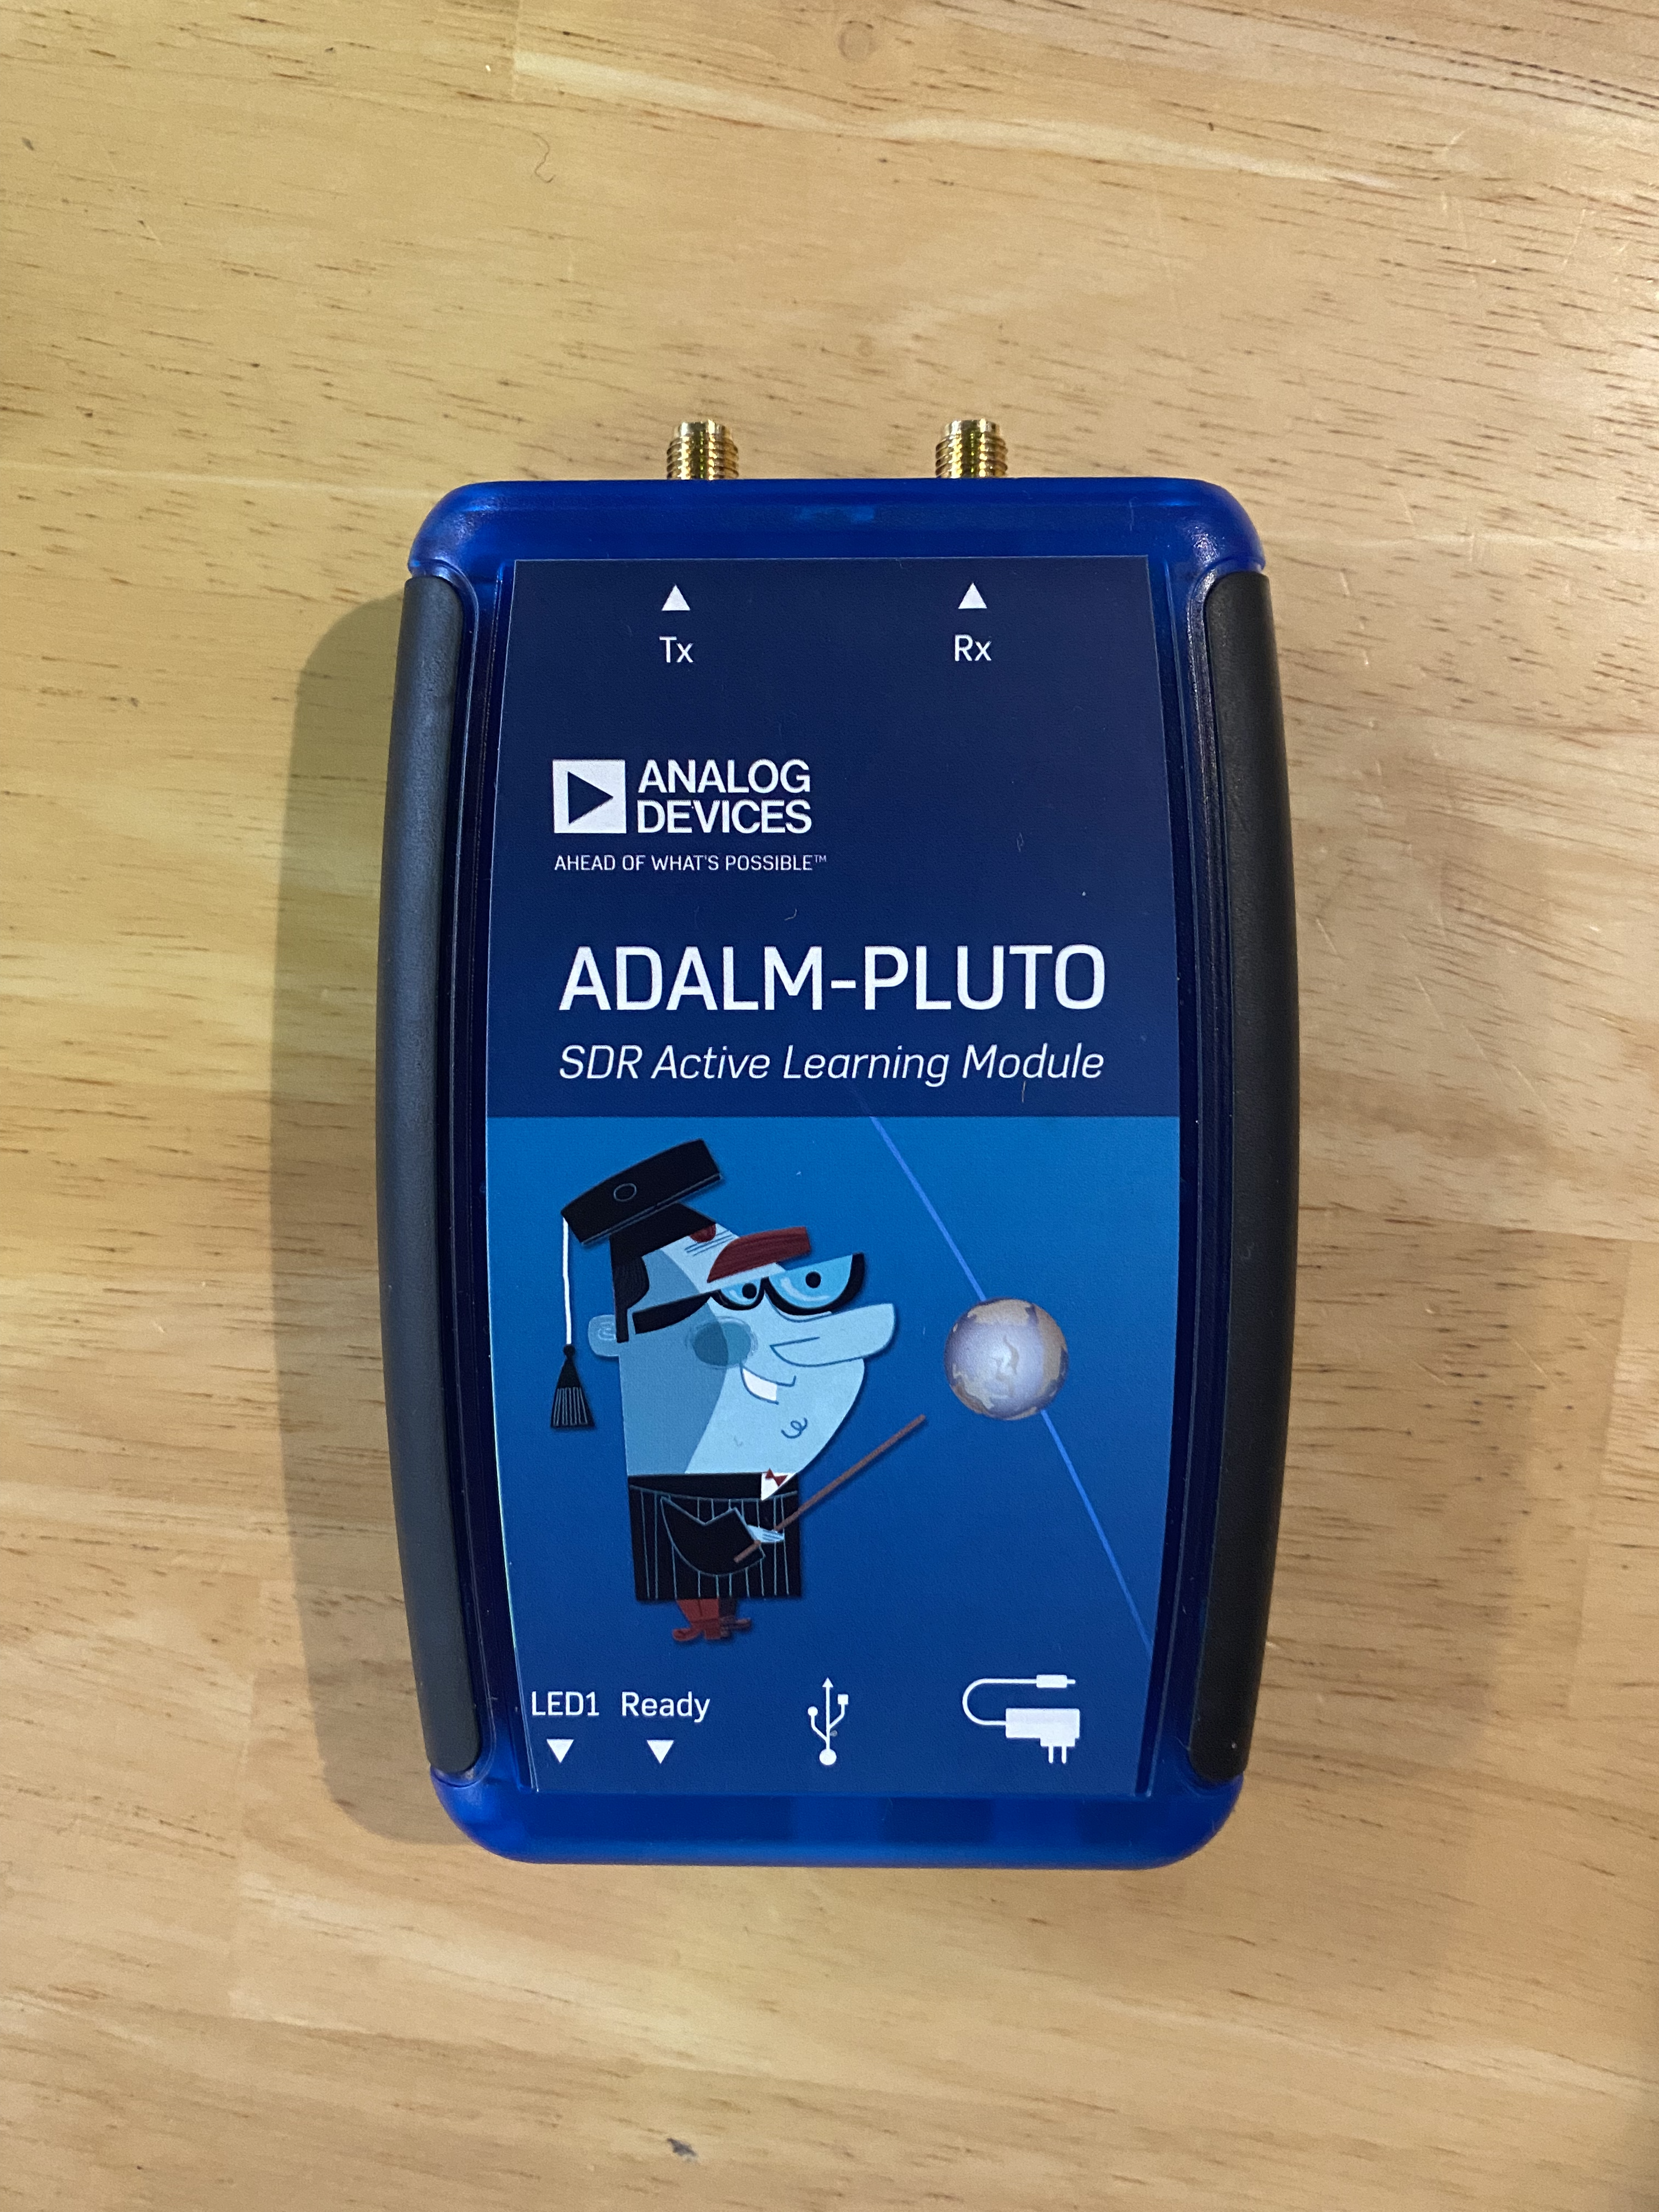
\includegraphics[scale=0.5, width=50mm]{images/pluto.png}
    \caption{Pluto au naturel}
    \label{fig:pluto}
\end{figure}

\begin{figure}
    \centering
    \includegraphics[scale=0.5, width=50mm]{images/hard_wired_sma.pdf}
    \caption{Pluto kit SMA male-male connector}
    \label{fig:sma}
\end{figure}

\begin{figure}
    \centering
    \includegraphics[scale=0.5, width=50mm]{images/pluto_antennas.pdf}
    \caption{Pluto kit antennas}
    \label{fig:ant}
\end{figure}

\newpage
\subsection{Lab Activity}
We will install the necessary software components, run an example transmit-and-receive (tx and rx, respectively) script, and test a few communication links.

\subsubsection{Equipment}
\begin{itemize}
    \item pluto kit
    \item laptop with MATLAB and Simulink
\end{itemize}

\subsubsection{Procedure}
Be sure to document your findings (pictures and screenshots) along the way for your lab notebook. 
\begin{itemize}
    \item Sign into \href{https://www.mathworks.com/}{MathWorks. }
    \item Install \href{https://www.mathworks.com/products/get-matlab.html?s_tid=gn_getml}{MATLAB } if you don't already have it on your machine.
    \item Install the \href{https://www.mathworks.com/hardware-support/adalm-pluto-radio.html}{ADALM-PLUTO Radio Support from Communications Toolbox. }
    \item Follow the hardware installation and connect the pluto to your computer via USB.
    \item Open MATLAB and hack your pluto by running the following line in the command window:
    \begin{lstlisting}[style=Matlab-editor, numbers=none]
    configurePlutoRadio('AD9364')
    \end{lstlisting}
  This will expand the operating frequency range by configuring the pluto to the AD9364 RF transceiver architecture which supports frequency tuning from 70 MHz to 6 GHz. The pluto by default will follow the AD9363 architecture which has the advertised operating range of 325 MHz to 3.8 GHz. 
    \item Verify that the \href{https://github.com/rjmacaranas/ee-504/blob/main/lab1/pluto_tx_and_rx.m}{receive-and-transmit MATLAB script } works. 
\end{itemize}

\subsubsection{Deliverables}
Document your set-up and results in your lab notebook and post next week before class.
\begin{enumerate}
    \item (25 pts) Screenshot of transmitted signal from tx-and-rx example MATLAB script.
    \item (25 pts) Screenshot of spectrum analyzer output from tx-and-rx with bare RF ports.
    \item (25 pts) Screenshot of spectrum analyzer output from tx-and-rx with a hard-wire link.
    \item (25 pts) Screenshot of spectrum analyzer output from tx-and-rx with an antenna air link.
\end{enumerate} 




\newpage
\section{FM, Nyquist, and Antennas}
\textit{``\href{https://en.wikipedia.org/wiki/Guglielmo_Marconi}{Marconi }plays the mamba, listen to the radio''}--- Starship.

\setcounter{subsection}{-1}

\subsection{Learning Objective}
The purpose of this session is to introduce the software-defined radio (SDR) unit that will be used in this course, review concepts of frequency modulation (FM), implement an FM receiver in software, construct an antenna, and measure the antenna gain performance.

\subsection{Before the Lab Session} 
Complete the following (can be done in parallel):
\begin{enumerate}
    \item Read all sections up to the lab activity.
    \item Install MATLAB, Simulink, and the ADALM-PlutoSDR support package onto your machine. There is a getting started video available on Canvas.

\end{enumerate}



\subsection{FM Theory}
Imagine you are at a party. Music is playing, everyone is either laughing, talking, or screaming across the room, and it seems impossible to have an intelligible conversation. You want to talk to your friend so you walk over to another room with them where it is quieter. Well this is the same idea behind signal modulation. We just walk our \textbf{message} to a different space in the frequency spectrum. The \textbf{carrier frequency} of our modulated signal is where we want to stand. A \textbf{channel} is the room that we are in which is inside some building, or \textbf{frequency band}. The \textbf{bandwidth} of our message is the range (varying timbre) of our voices. You and your friend can hear all the people in the party room still so their bandwidth extends the \textbf{guardband}, walls, and  prohibits complete \textbf{channel separation}. FM is one technique we can use to relocate our message.

\begin{figure}
    \centering
    \includegraphics[scale=0.5, width=175mm]{images/United_States_Frequency_Allocations_Chart_2016_-_The_Radio_Spectrum.pdf}
    \caption{United States Frequency Allocations, \href{https://www.fcc.gov/engineering-technology/policy-and-rules-division/general/radio-spectrum-allocation}{Federal Communications Commission (FCC)}}
    \label{fig:RF}
\end{figure}

\subsubsection{Definition}
We define an FM signal as Eq. \ref{FM}. Modulated signals are typically represented as $\phi(t)$ with some subscript describing the nature of modulation. An FM signal can be described as a sinusoid with constant carrier amplitude and time-varying frequency that is proportional to some integral gain of the message signal.


\begin{equation} \label{FM}
    \phi_{FM}(t) = A_c \cos \Big{[}\omega_ct + k_f \int_{-\infty}^{t} m(\lambda) d \lambda \Big{]}
\end{equation}

\subsubsection{Modulation Index}
The FM modulation index $\beta$, also known as the frequency deviation ratio, is defined as the ratio of the frequency deviation, of the modulated signal, to the message signal bandwidth as given by Eq. \ref{FM mod}. The frequency deviation describes how far our modulated signal can be displaced from the carrier which effectively constrains the spectrum.

\begin{equation} \label{FM mod}
    \beta = \frac{\Delta f}{B} = \frac{\Delta \omega}{2\pi B}
\end{equation}

\subsection{Antenna Theory}
We are not going to worry too much about antenna theory here since this is a study of software-defined radio. You might notice that the antennas provided in your kit are fairly small. There are many types of antenna and in general the length of an antenna is inversely proportional to its intended operation frequency. Recall that the frequency operating range of plutos goes from 324 MHz to 3.8 GHz. The antennas that are provided in our kit were designed for the range of operation specified, but we want to \textit{hack} the pluto to go to the lower frequency FM broadcast band. We might achieve better performance by creating an antenna that is designed for the lower frequency. There are a number of different antenna parameters that we can measure to characterize  performance such as: gain, bandwidth, radiation pattern, polarization, and impedance. You should have some familiarity with gain  and impedance concepts from prerequisite coursework, so we will stick to observing gain in the frequency spectrum and impedance in the antenna construction. 

\subsubsection{Whip Antenna}
We will create a whip, or monopole, antenna. Recall from circuit theory that maximum power transfer occurs when the impedance of the source and load are matched. For a monopole topology, we can approximate an impedance inverter by creating an antenna that is of quarter-wave length, $\lambda/4$, for reasons that are beyond the scope of this class (electromagnetism and our good friend Maxwell). The quarter-wave length of our monopole antenna is given in meters by Eq. (\ref{ant-len}) where $f$ is our target frequency in Hertz and $c$ is the speed of light, approximately $3\times10^{9} m/s$.

\begin{equation} \label{ant-len}
    l = \frac{f/4}{c} (meters)
\end{equation}

There is a ten-week treatment of antenna theory offered at Cal Poly, EE 533 usually taught by Professor Arakaki in the spring, if you are interested in expanding your mind.
\subsubsection{Antenna Construction}
The antenna that I intend for us to design is composed of an insulated copper wire soldered to the center conductor of an SMA female connector. The copper wire is cut to a length such that the total length of hard-wire link and copper wire matches the monopole quarter-wave antenna length. Again this is probably not the greatest antenna ever made, but it does a fair job of showing us the importance of the length of an antenna. My whip antenna is shown in Figure \ref{fig:whip}.

\begin{figure}
    \centering
    \includegraphics[scale=0.5, width=40mm]{images/whip.png}
    \caption{Whip antenna construction}
    \label{fig:whip}
\end{figure}

\subsection{Nyquist and Sampling Theorem}
You should know by know that if we do not sample a signal at least twice the highest frequency present then we introduce the possibility for aliasing. In the frequency spectrum, this manifests itself as a remapping of content. To observe this effect, we will downsample the received signal until we notice changes in the frequency spectrum. Due to signal processing constraints, I have provided a Simulink model to capture the signal and a separate model for the spectrum analysis.

\newpage
\subsection{Lab Activity}
We will create an FM broadcast receiver using a pluto, MATLAB, Simulink, one of the provided antennas, and a whip antenna that you create. Our target frequency will be Cal Poly's radio station KCPR, which is 91.3 FM in the San Luis Obispo area and has a carrier of 91.3 MHz.

\subsubsection{Equipment}
\begin{itemize}
    \item pluto kit
    \item laptop with MATLAB and Simulink
    \item SMA connector and insulated copper wire
    \item solder and soldering station
\end{itemize}

\subsubsection{Procedure}
Be sure to document your findings (pictures and screenshots) along the way for your lab notebook. 
\begin{itemize}
    \item Connect the antenna from your kit to the Rx port of your pluto.
    \item Download and open the example FM capture Simulink model.
    \item Double-click the ADALM-PLUTO Receiver and tune the center frequency to KCPR.
    \item Lower the volume on your device so as to not damage your speakers and ears. 
    \item Run the program and observe audio fidelity of the pluto kit antenna for FM band receiving.
    \item Determine the antenna length for a whip antenna optimized for 91.3 MHz, cut a piece of wire to approximately that length, and solder it onto the center conductor of an SMA.
    \item Connect your whip antenna to the Rx port and try running the Simulink model again.
    \item Try to get a good audio sample to use for spectrum analysis.
    \item Using the FM baseband plotter model, adjust the downsample factor until aliasing occurs.
    \item Discuss your findings in your lab notebook (set-up, results, conclusion).
\end{itemize}

\subsubsection{Deliverables}
\begin{enumerate}
    \item (25 pts) Whip antenna length calculation and picture of hardware set-up with whip antenna.
    \item (25 pts) Comparison of audio fidelity between antennas. You can tune in to KCPR \href{https://kcpr.org/}{here.}
    \item (25 pts) Spectrum analyzer screenshot of original signal and of aliased signal. 
    \item (25 pts) Feedback on the activity. Maybe there is something that you want changed or you came up with a simple hack that improved antenna performance. Or maybe you found the assignment fun, or too short/long.
\end{enumerate} 


\end{document}